\documentclass[10pt, twoside]{article}
\usepackage{main}

% Aquí empieza el documento{{{
\begin{document}

%\maketitle
\thispagestyle{fancy}

\textbf{Alberto Oporto Ames \#139}

\section{Preguntas}%
\label{sec:preguntas}

\begin{enumerate}
	\setcounter{enumi}{1}
	\item Se coloca una lámina de cobre sobre el polo de un electroimán,
		con el campo magnético perpendicular a la lámina.
		Cuando se tira de la lámina hacia afuera,
		se requiere una fuerza considerable,
		la cual aumenta con la rapidez.
		Explica este fenómeno.
		\subitem La fuerza es proporcional a la rapidez a la que la lámina
			se aleja del electronimán.
	\setcounter{enumi}{3}
	\item Cuando un imán se suelta dentro de un tubo cobre,
		este caerá más lentamente que si fuerza soltado fuera del tubo.
		Si el cobre no es un material ferromagnético,
		¿Por qué ocurre esto?
		\subitem Porque la $fem$ de las cargas del tubo crea un
			campo magnético en sentido contrario a el del imán.
	\item Un avión vuela horizontalmente sobre la Antártida,
		donde el campo magnético terrestre está dirigido sobre todo hacia el
		frente del avión,
		¿el extremo del ala izquierda está a un potencial mayor que el del ala
		derecha?
		¿La respuesta depende de la dirección en que vuela el avión?
		\subitem No.
		\subitem Sí, si es que gira $90°$ a la derecha.
\end{enumerate}

\section{Problemas}%
\label{sec:problemas}

\begin{enumerate}
	\item Halla el flujo magnético sobre la superficie lateral para cada uno
		de los siguientes sólidos.
		Considera que la magnitud del campo magnético uniforme y constante de
		$B$ es $1mT$.
		\begin{enumerate}
			\item Una pirámide cuyas caras son triángulos equiláteros de
				$0.5m$ de lado.
		\end{enumerate}
		\begin{figure}[H]
			\centering
			\begin{tikzpicture}[scale=1, transform shape]
				\begin{scope}[canvas is xz plane at y=0]
					% La base
					\node (algo) at (0,0) [shape=rectangle, draw, minimum size=3cm] {};
				\end{scope}

				% Las aristas de los lados de la pirámide
				\draw(0,3,0) -- (algo.north west);
				\draw(0,3,0) -- (algo.north east);
				\draw(0,3,0) -- (algo.south east);
				\draw(0,3,0) -- (algo.south west);

				% Las esquinas
				\draw (algo.north west) node[below] {$P$};
				\draw (algo.north east) node[below] {$S$};
				\draw (algo.south east) node[right] {$R$};
				\draw (algo.south west) node[below] {$Q$};

				% La longitud de los lados de la base
				\draw (algo.north) node[above] {$0.5m$};
				\draw (algo.east)++(0.25,0) node[right] {$0.5m$};

				% El campo magnético
				\draw[-{Latex[length=5]}] (-3,2) -- ++(0,-2)
					node [midway, right] {$\vec{B}$};
			\end{tikzpicture}
		\end{figure}
		\[
			\phi = 4AB\cos{\alpha}
		\]
		\begin{figure}[H]
			\centering
			\begin{tikzpicture}[scale=1, transform shape]
				\node (tri) at (0,0)
					[
						regular polygon,
						regular polygon sides=3,
						%
						draw,
						minimum size=3cm
					]
					{};
				\draw (tri.south) -- (tri.north)
					node [midway, right] {$L$};

				\draw (tri.side 1) node [left] {$0.5m$};
				\draw (tri.side 2) node [below] {$0.5m$};
				\draw (tri.side 3) node [right] {$0.5m$};

			\end{tikzpicture}
		\end{figure}
		\begin{align*}
			A &= 0.25m*L\\
			\\
			L &= (0.5) \frac{\sqrt{3}}{2}m\\
			\\
			A &= \frac{\sqrt{3}}{16}m\\
		\end{align*}
		\begin{figure}[H]
			\centering
			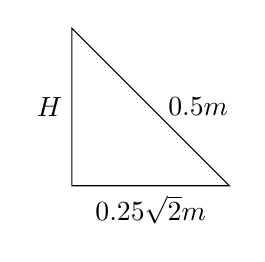
\begin{tikzpicture}[scale=1, transform shape]
				\coordinate (A) at (0,0);
				\coordinate (B) at (2,0);
				\coordinate (C) at (0,2);
				\draw (A) -- (B)
					node [midway, below] {$0.25\sqrt{2}m$}
					-- (C)
					node [midway, right=0.1cm] {$0.5m$}
					-- cycle
					node [midway, left] {$H$}
					;
			\end{tikzpicture}
		\end{figure}
		\begin{figure}[H]
			\centering
			\begin{tikzpicture}[scale=1, transform shape]
				\coordinate (A) at (0,0);
				\coordinate (B) at (3,0);
				\coordinate (C) at (0,3);
				\draw (A) -- (B)
					node [midway, below] {$0.25\sqrt{2}m$}
					-- (C)
					node [midway, right=0.1cm] {$0.5m$}
					-- cycle
					node [midway, left] {$0.25\sqrt{2}m$}
					pic [pic text=$\beta$, draw, angle radius=1cm] {angle=C--B--A}
					pic [pic text=$\alpha$, draw, angle radius=1cm] {angle=A--C--B}
					;
			\end{tikzpicture}
		\end{figure}
		\[
			\alpha = 45°
		\]
		\begin{align*}
			\phi &= 4* \frac{\sqrt{3}}{16}m *1mT* \cos{45°}\\
			\phi &= 4* \frac{\sqrt{3}}{16}m *1mT* \frac{\sqrt{2}}{2} \\
			\phi &= \frac{\sqrt{6}}{8}mWb
		\end{align*}
	\setcounter{enumi}{3}
	\item Dos espiras circulares se sitúan de la manera mostrada en la figura.
		La espira superior posee una intensidad de corriente de valor $I$,
		mientras que la espira inferior se encuentra desconectada.
		Si la espira superior se mueve hacia arriba, determina:
		\begin{figure}[H]
			\centering
			\begin{tikzpicture}[scale=1, transform shape]
				\begin{scope}[canvas is xz plane at y=0]
					\draw (0,0) circle (2);
				\end{scope}
				\begin{scope}[canvas is zx plane at y=0.5]
					%\draw (0,0) circle (2);
					%\draw (0:2) arc ()
					\draw[-{Latex[length=5]}] (0:2) arc (0:360:2);
				\end{scope}
					\node at (180:1) {$I$};
			\end{tikzpicture}
		\end{figure}

		\begin{enumerate}
			\item La dirección de la corriente inducida en la espira inferior.
				\subitem Antihorario.
			\item La dirección de la fuerza magnética inducida en la espira inferior.
				\subitem Hacia arriba.
		\end{enumerate}
		Si se incrementa la corriente que pasa por la espira superior, determina:
		\begin{enumerate}
			\item La dirección de la corriente inducida en la espira inferior.
				\subitem Horario.
			\item La dirección de la fuerza magnética inducida en la espira inferior.
				\subitem Hacia abajo.
		\end{enumerate}
	\setcounter{enumi}{6}
	\item Dado el circuito mostrado en la figura, que consta de un circuito
		circula conectado a una fuente de voltaje $V$ y resistencia $R$,
		una espira circular en el interior de circuito y otra espira
		en su exterior; determina:
		\begin{figure}[H]
			\centering
			\begin{tikzpicture}
				[
					scale=1,
					transform shape,
					circuit ee IEC,
					set resistor graphic=var resistor IEC graphic
				]
				\draw (0,2) to [make contact={info={S}}](1,2);

				\draw (0,0) to [resistor] (0,1.5)
					to [battery={xscale=-1}] (0,2);

				\draw (0,0) -- (1,0);

				\draw (1,2) arc (135:-135:{sqrt(2)});

				\draw (2,1) circle (0.5);
				\draw (5,1) circle (0.5);

			\end{tikzpicture}
		\end{figure}

		\begin{enumerate}
			\item La dirección de la corriente inducida en cada uno de los
				anillos circulares cuando el interruptor ``$S$'' es
				cerrado súbitamente.
		\end{enumerate}
		\begin{figure}[H]
			\centering
			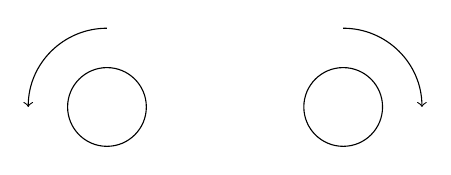
\begin{tikzpicture}
				%\draw (0,2) to [make contact={info={S}}](1,2);

				%\draw (0,0) to [resistor] (0,1.5)
				%	to [battery={xscale=-1}] (0,2);

				%\draw (0,0) -- (1,0);

				%\draw (1,2) arc (135:-135:{sqrt(2)});

				\draw (2,1) circle (0.5);
				\draw [->] (2,1)
					+(90:1) arc (90:180:1);

				\draw (5,1) circle (0.5);
				\draw [->] (5,1)
					+(90:1) arc (90:0:1);

			\end{tikzpicture}
		\end{figure}
	\setcounter{enumi}{10}
	\item En la figura se observa una espira circular de radio $R(5mm)$ ubicada
		a una distancia $r(50cm)$ de un alambre recto muy largo por el cual
		circula una corriente $I$ que varía con el tiempo $t$ de acuerdo con
		la gráfica mostrada.
		Determina:
		\begin{figure}[H]
			\centering
			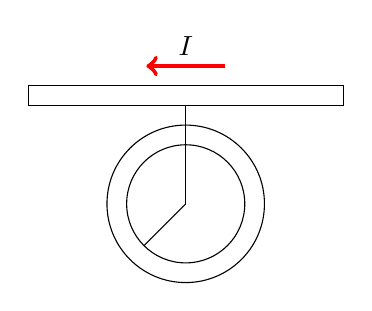
\begin{tikzpicture}[scale=1, transform shape]

				\draw (-2,1.25) rectangle ++(4,0.25);

				\draw[->, ultra thick, red] (0.5,1.75) -- ++(-1,0);

				\node at (0,2) {$I$};

				% Aro
				\draw (0,0) circle (0.75);
				\draw (0,0) circle (1);

				\draw (0,0) -- ++(-135:0.75);
				\draw (0,0) -- ++(0,1.25);

			\end{tikzpicture}
		\end{figure}
		\begin{figure}[H]
			\centering
			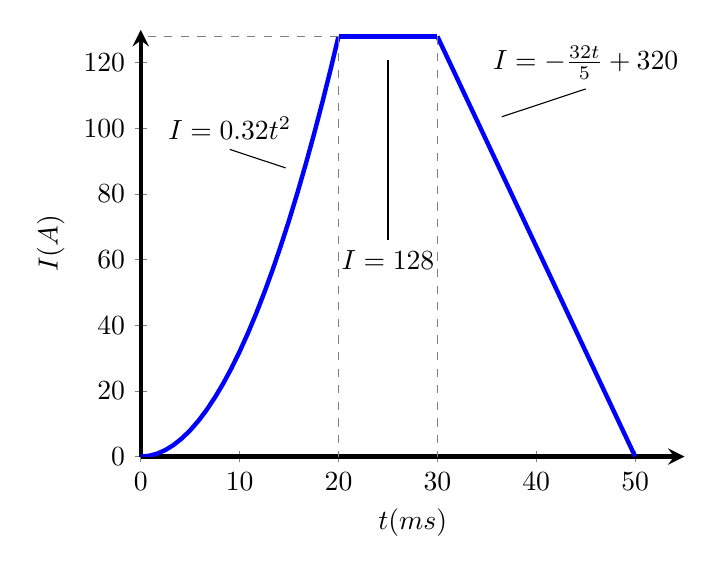
\begin{tikzpicture}[scale=1, transform shape]
				\begin{axis}
					[
						width=0.7\linewidth,
						height=7cm,
						%
						ymin=0,
						ymax=130,
						%
						xmin=0,
						xmax=55,
						%
						axis y line=left,
						axis x line=bottom,
						axis line style = ultra thick,
						%
						xlabel={$t(ms)$},
						ylabel={$I(A)$}
					]
					\addplot
						[
							domain={0:20},
							blue,
							ultra thick
						]
						{0.32*x^2};
					\addplot
						[
							domain={20:30},
							blue,
							ultra thick
						]
						{128};
					\addplot
						[
							domain={30:50},
							blue,
							ultra thick
						]
						%{(-128*(x-50)/20)};
						{320-32*x/5};

					%\coordinate (inicioPlano) at (20,128);
					%\coordinate (inicioPlanox) at (20,0);
					%\coordinate (inicioPlanoy) at (0,128);

					\draw[gray, dashed] (20,128) -- (0,128);

					\draw[gray, dashed] (20,128) -- (20,0);
					\draw[gray, dashed] (30,128) -- (30,0);

					\node (algo) at (9,100) {$I=0.32t^2$};
					\draw (algo.south) -- ++(-45:8);

					\node (algo2) at (25,60) {$I=128$};
					\draw (algo2.north) -- ++(0,55);

					\node (algo3) at (45,120) {$I=- \frac{32t}{5} +320$};
					\draw (algo3.south) -- ++(-135:12);
				\end{axis}
			\end{tikzpicture}
		\end{figure}

		\begin{enumerate}
			\item La corriente inducida en el instante $t=15ms$.
				\begin{align*}
					\mathcal{E} &= - \frac{d\phi}{dt} \\
					\\
					\phi &= AB\cancel{\cos{\theta}}\\
					\\
					A &= 25\pi*10^{-6}m \\
					B &= 4I*10^{-7}\\
					\\
					\phi  & = I\pi*10^{-11}\\
					d\phi & = \pi*10^{-11}dI\\
					\\
					\frac{dI}{dmt} &=
					\begin{cases}
						0.64t          & 0 \leq t \leq 20\\
						0              & 20 < t \leq 30\\
						- \frac{32}{5} & 30 < t \leq 50
					\end{cases}\\
					\\
						\mathcal{E} &= -\pi*10^{-11} * \frac{dI}{dt}\\
						\mathcal{E} &= -\pi*10^{-11} * 1000\frac{dI}{dmt}\\
						\mathcal{E} &= -\pi*10^{-11} * 1000*(0.64*15)A\\
						\mathcal{E} &= - 9.6\pi*10^{-8}A
				\end{align*}
			\item El flujo magnético en el instante $t=40ms$.
				\begin{align*}
					\phi &= I\pi*10^{-11}\\
					\phi &= ( -\frac{32*40}{5}+320 )\pi*10^{-11}\\
					\phi &= 64\pi*10^{-11} Wb
				\end{align*}
			\item La fem inducida en el instante $t=10ms$.
				\begin{align*}
					\mathcal{E} &= -\pi*10^{-11} * 1000\frac{dI}{dmt}\\
					\mathcal{E} &= -\pi*10^{-11} * 1000*(0.64*10)A\\
					\mathcal{E} &= - 6.4\pi*10^{-8}A
				\end{align*}
			\item La dirección de la corriente inducida para todo instante.
				\begin{align*}
					\begin{cases}
						\text{Horario}     & 0 \leq t \leq 20\\
						\cancel{O}         & 20 < t \leq 30\\
						\text{Antihorario} & 30 < t \leq 50
					\end{cases}
				\end{align*}
			\item La gráfica de fem inducida vs. tiempo.

			\begin{figure}[H]
			\centering
			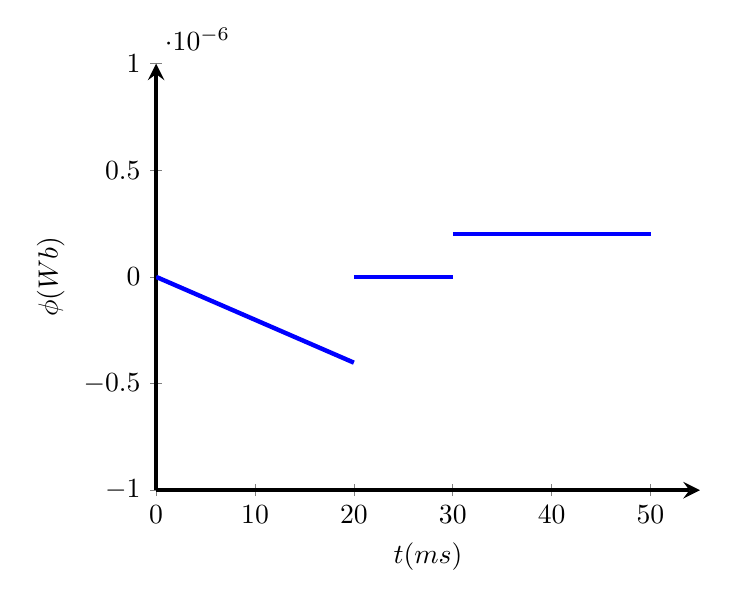
\begin{tikzpicture}[scale=1, transform shape]
				\begin{axis}
					[
						width=0.7\linewidth,
						height=7cm,
						%
						ymin=-0.000001,
						ymax=0.000001,
						%
						xmin=0,
						xmax=55,
						%
						axis y line=left,
						axis x line=bottom,
						axis line style = ultra thick,
						%
						xlabel={$t(ms)$},
						ylabel={$\phi(Wb)$}
					]
					\addplot
						[
							domain={0:20},
							blue,
							ultra thick
						]
						{-pi*10^(-11)*1000*(0.64*x)};
					\addplot
						[
							domain={20:30},
							blue,
							ultra thick
						]
						{0};
					\addplot
						[
							domain={30:50},
							blue,
							ultra thick
						]
						{-pi*10^(-11)*1000*(-32/5)};

				\end{axis}
			\end{tikzpicture}
		\end{figure}
		\end{enumerate}
\end{enumerate}

\vfill
Código fuente: \url{https://github.com/otreblan/fisi-2-tarea-6}

\end{document}
%}}}
